\section{\texorpdfstring{$D^0$}{d0} Decays}
\paragraph{a)}
\begin{figure}[H]
	\centering
	\begin{subfigure}{0.49\textwidth}
		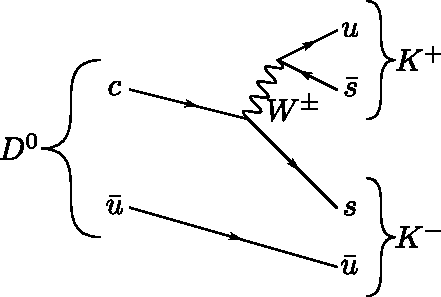
\includegraphics[width=\textwidth]{figures/D0_K+K-.pdf}
		\caption{$D^0 \to K^+ K^-$}
	\end{subfigure}
	\hfill
	\begin{subfigure}{0.49\textwidth}
		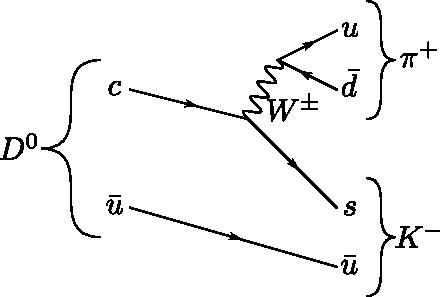
\includegraphics[width=\textwidth]{figures/D0_K-pi+.pdf}
		\caption{$D^0 \to K^- \pi^+$}
	\end{subfigure}
	\caption{Feynman diagrams for the decays $D^0 \to K^+ K^-$ and $D^0 \to K^- \pi^+$.}
\end{figure}

The only vertex that differs between these decays are the $\bar{s} u W^\pm$-vertex and the $\bar{d} u W^\pm $-vertex. The CKM matrix elements are $\abs{V_{us}} = \num{0.2243(8)}$ and $\abs{V_{ud}} = \num{0.97373(31)}$. Thus
\begin{equation}
	\frac{\Gamma(D^0 \to K^+ K^-)}{\Gamma(D^0 \to K^- \pi^+)} = \frac{\abs{V_{us}}^2}{\abs{V_{ud}}^2} = \num{0.0531(4)},
\end{equation}
and the value found in \cite{particles} is \num{0.1033(13)}, which is a ratio of \SI{51.4(7)}{\percent}.

\paragraph{b)}
\begin{figure}[H]
	\centering
	\begin{subfigure}{0.49\textwidth}
		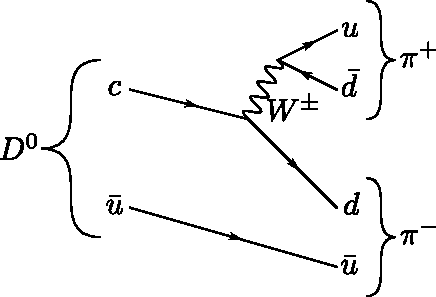
\includegraphics[width=\textwidth]{figures/D0_pi+pi-.pdf}
		\caption{$D^0 \to \pi^+ \pi^-$}
	\end{subfigure}
	\hfill
	\begin{subfigure}{0.49\textwidth}
		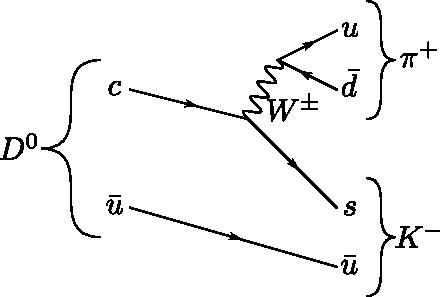
\includegraphics[width=\textwidth]{figures/D0_K-pi+.pdf}
		\caption{$D^0 \to K^- \pi^+$}
	\end{subfigure}
	\caption{Feynman diagrams for the decays $D^0 \to \pi^+ \pi^-$ and $D^0 \to K^- \pi^+$.}
\end{figure}
The only vertex that differs between these decays are the $c d W^\pm$-vertex and the $c s W^\pm$-vertex. The CKM matrix elements are $\abs{V_{cd}} = \num{0.221(4)}$ and $\abs{V_{cs}} = \num{0.975(6)}$. Thus
\begin{equation}
	\frac{\Gamma(D^0 \to \pi^+ \pi^-)}{\Gamma(D^0 \to K^- \pi^+)} = \frac{\abs{V_{cd}}^2}{\abs{V_{cs}}^2} = \num{0.0514(20)},
\end{equation}
and the value found in \cite{particles} is \num{0.0368(5)} which is a ratio of \SI{140(6)}{\percent}

\paragraph{c)}
\begin{figure}[H]
	\centering
	\begin{subfigure}{0.49\textwidth}
		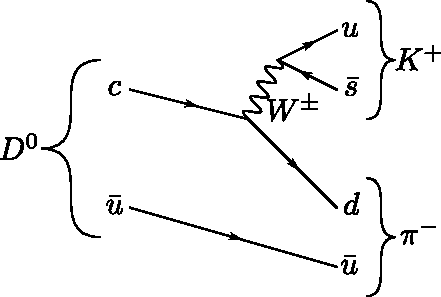
\includegraphics[width=\textwidth]{figures/D0_K+pi-.pdf}
		\caption{$D^0 \to K^+ \pi^-$}
	\end{subfigure}
	\hfill
	\begin{subfigure}{0.49\textwidth}
		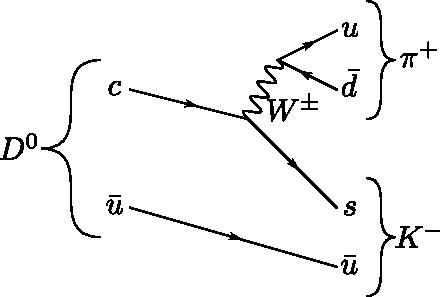
\includegraphics[width=\textwidth]{figures/D0_K-pi+.pdf}
		\caption{$D^0 \to K^- \pi^+$}
	\end{subfigure}
	\caption{Feynman diagrams for the decays $D^0 \to K^+ \pi^-$ and $D^0 \to K^- \pi^+$.}
\end{figure}
The vertices that differs are the $u \bar{s} W^\pm$-vertex, $u \bar{d} W^\pm$-vertex, $c d W^\pm$-vertex, and $c s W^\pm$-vertex. The CKM matrix elements are mentioned in a) and b). Thus
\begin{equation}
	\frac{\Gamma(D^0 \to K^+ \pi^-)}{\Gamma(D^0 \to K^- \pi^+)} = \frac{\abs{V_{cd}}^2 \times \abs{V_{us}}^2}{\abs{V_{cs}}^2 \times \abs{V_{ud}}^2} = \num{0.00273(11)},
\end{equation}
and the value found in \cite{particles} is \num{0.00379(18)} which is a ratio of \SI{72(4)}{\percent}.